\documentclass[usenames,dvipsnames]{include/protokollclass}
% Main File - Based on protokollclass.cls
% Comments are mostly in English (and some in German, concerning the Praktikum)
% ------------------------------------------------------------------------------
% Further files in folder:
%  - include/cmds.tex (for macros and additional commands)
%  - include/kitlogo.pdf (for titlepage)
%  - lit.bib (bibtex bibliography database)
%  - include/titlepage.tex (for layout of titelpage)
% ------------------------------------------------------------------------------
% Useful Supplied Packages:
% amsmath, amssymb, mathtools, bbm, upgreek, nicefrac,
% siunitx, varioref, booktabs, graphicx, tikz, multicol







\usepackage{siunitx}
\usepackage{tikz}
\usepackage{subfigure}

\usepackage{xargs}                      % Use more than one optional parameter in a new commands
\usepackage{xcolor}  % Coloured text etc.
% 
\usepackage[colorinlistoftodos,prependcaption,textsize=tiny]{todonotes}
\newcommandx{\unsure}[2][1=]{\todo[linecolor=red,backgroundcolor=red!25,bordercolor=red,#1]{#2}}
\newcommandx{\change}[2][1=]{\todo[linecolor=blue,backgroundcolor=blue!25,bordercolor=blue,#1]{#2}}
\newcommandx{\info}[2][1=]{\todo[linecolor=OliveGreen,backgroundcolor=OliveGreen!25,bordercolor=OliveGreen,#1]{#2}}
\newcommandx{\improvement}[2][1=]{\todo[linecolor=Plum,backgroundcolor=Plum!25,bordercolor=Plum,#1]{#2}}
\newcommandx{\thiswillnotshow}[2][1=]{\todo[disable,#1]{#2}}

%% --------------------------------------
%% |    Settings for Word Separation    |
%% --------------------------------------
% Help for separation:
% In German package the following hints are additionally available:
% "- = Additional separation
% "| = Suppress ligation and possible separation (e.g. Schaf"|fell)
% "~ = Hyphenation without separation (e.g. bergauf und "~ab)
% "= = Hyphenation with separation before and after
% "" = Separation without a hyphenation (e.g. und/""oder)

% Describe separation hints here:
\hyphenation
{
    über-nom-me-nen an-ge-ge-be-nen
    %Pro-to-koll-in-stan-zen
    %Ma-na-ge-ment  Netz-werk-ele-men-ten
    %Netz-werk Netz-werk-re-ser-vie-rung
    %Netz-werk-adap-ter Fein-ju-stier-ung
    %Da-ten-strom-spe-zi-fi-ka-tion Pa-ket-rumpf
    %Kon-troll-in-stanz
}





% um die Titelseite per PDF-reader auszufüllen. Vorgefertigte Daten
% können in Datei 'data.tex' modifiziert werden.
%\setboolean{forminput}{true}
% um die Anmerkungen zu den Textfeldern anzeigen zu lassen
%\setboolean{showannotations}{true}
% Erneuern der Seitenzahl in jedem Kapitel
%\setboolean{chapResetPageNumb}{true}
% Einbinden der Kapitelnummer in der Seitenzahl
%\setboolean{chapWiseNumb}{true}
% english or ngerman (new german für neue deutsche Rechtschreibung statt german)
\SelectLanguage{ngerman}

%% ---------------------------------------------
%% |    Informationen über dieses Protokoll    |
%% ---------------------------------------------
\newcommand{\praktikum}{}                % P1 oder P2
\newcommand{\semester}{}            % z.B. "WS14/15" oder "SS15"

\newcommand{\wochentag}{}                % Mo, Di, Mi oder Do
\newcommand{\gruppennr}{}                % Zweistellige Gruppennummer

\newcommand{\nachnamea}{}             % Nachname des ersten Praktikanten
\newcommand{\vornamea}{}               % Vorname des ersten Praktikanten
\newcommand{\nachnameb}{}              % Nachname des zweiten Praktikanten
\newcommand{\vornameb}{}              % Vorname des zweiten Praktikanten

\newcommand{\emailadressen}{}
% optionale Angabe von Emailadresse(n) für den Kontakt mit dem Betreuer

\newcommand{\versuch}{} % Name des Versuchs
\newcommand{\versuchsnr}{}               % bitte die korrekte Nummer dem 
% Arbeitsplatz am Versuchstag 
% entnehmen
\newcommand{\fehlerrechnung}{}         % Ob Fehlerrechnung im Versuch 
% durchgeführt wurde oder nicht

\newcommand{\betreuer}{}      % Name des zuständigen Betreuers
\newcommand{\durchgefuehrt}{}      % Datum, an dem der Versuch 
% durchgeführt wurde

%% -----------------------
%% |    Main Document    |
%% -----------------------
\begin{document}
    % Titlepage und ToC
    \FrontMatter
\begin{titlepage}


\end{titlepage}

    \begingroup \let\clearpage\relax    % in order to avoid listoffigures and
    \tableofcontents                    % listoftables on new pages
    \listoffigures
    \listoftables
    \endgroup
    %\cleardoublepage



    % Contents
    \MainMatter
    
    %\emptychapter[1]{Messprotokoll 1}{} % usage: \emptychapter[page displayed 
                                        %        in toc]{name of the chapter}
    %\pseudochapter[3]{Messprotokoll 2}  % usage: \pseudochapter[number of pages 
                                        %        added]{name of the chapter}
            
%    \setcounter{chapter}{-1}
%    \emptychapter[1]{Aufgabenstellung}{}
%    \includepdf[pages=1, 
%    pagecommand={\thispagestyle{fancy}}, 
%    offset=2.5cm -2.5cm]{./fig/fig_aufgabenblatt}
%
%    \includepdf[pages=2, 
%    pagecommand={\thispagestyle{fancy}}, offset=-2.5cm 
%    -0.5cm, trim=0cm 4cm 0cm 0cm, clip ]{./fig/fig_aufgabenblatt}
%
%	 \includepdf[pages=3, 
%    pagecommand={\thispagestyle{fancy}}, offset=2.5cm 
%    -0.5cm, trim=0cm 4cm 0cm 0cm, clip ]{./fig/fig_aufgabenblatt}
%
	
	\chapter{Versuchsaufbau und Alignment}
	Der Versuchsaufbau ist mehrere Schritte unterteilt.
	Die ersten Versuchstage beinhalteten den Aufbau der Messanordnung. Der experimentelle Aufbau ist in Abbildung \ref{fig:aufbau} dargestellt. Anschließend wurde eine Kalibrierung der Module durchgeführt. Mittels Software wurden alle kaputten Pixel von der Auswertung ausgeschlossen.
	An einem weiteren Versuchstag wurden der external trigger und die clock in pXar gesetzt.
	Außerdem wurde ein Latency Test zwischen Trigger und Detektormodulen durchgeführt.
	
	\begin{figure}
		\centering
		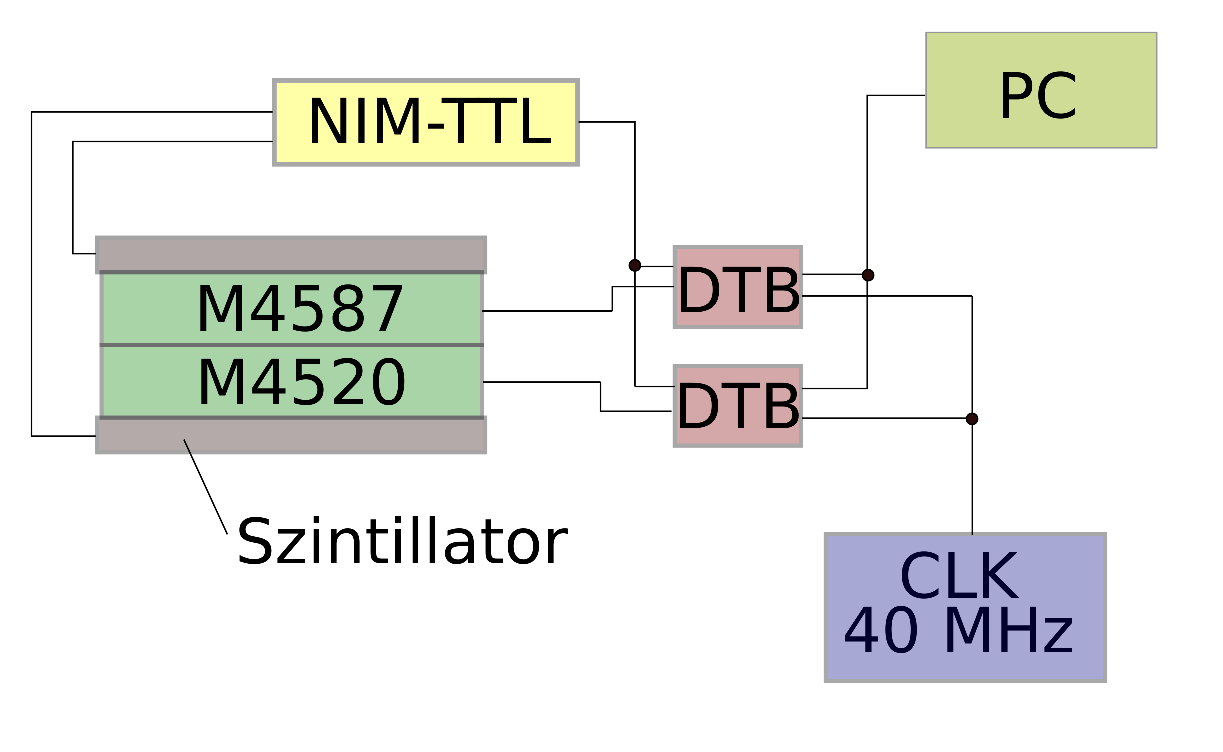
\includegraphics[width=0.7\textwidth]{fig/aufbau.eps}
		\caption{Die Module, die die Silizium Pixel enthalten sind von zwei Szintillatorzähler umgeben, die über eine Koinzidentsschaltung und eine Signalumwandlung die Triggersignale für die DTB's liefern. Die DTB's werden mit 40 MHz synchron über ein FPGA Board getaktet und werden über eine USB-Schnittstelle mit einem PC ausgelesen.}
		\label{fig:aufbau}
	\end{figure}

	\section{Latency Scan}
	\subsection{Mit aktiver Quelle}
	Zuerst wurde eine Langzeitmessung mit Latency im Bereich 0 - 150 gestartet. 
	Es gab mehrere Probleme mit den Registereinträgen beim Auslesen, deshalb wurde die Messung mit kosmischen Myonen wiederholt. 
	\subsection{Mit kosmischen Myonen}
	Hier wurde die Messung mit Latency im Bereich 68-83 durchgeführt und anschließend die Hitmaps ausgewertet. Dabei wurden Events mit Double Colum Error ignoriert. Die Messung mit einer Latency von 81 ergab die meisten Hits. Alle weiteren Messungen wurden mit dieser Latency durchgeführt.
	
	\section{Bestimmung der Ausrichtung zueinander}
	Zur Bestimmung der Ausrichtung der beiden Baords zueinander, wurde eine radioaktive Quelle an zwei unterschiedlichen Stellen über den Boards platziert. Die Durchnummerierung und die Lage der x und y Achse sind in Abbildung \ref{fig:board} dargestellt. Die Ergebnisse der Alignmentmessung mit den zwei unterschiedlichen Positionen der Quelle sind in Abbildung \ref{fig:alignment} a) und b) dargestellt.
	\begin{figure}
		\centering
		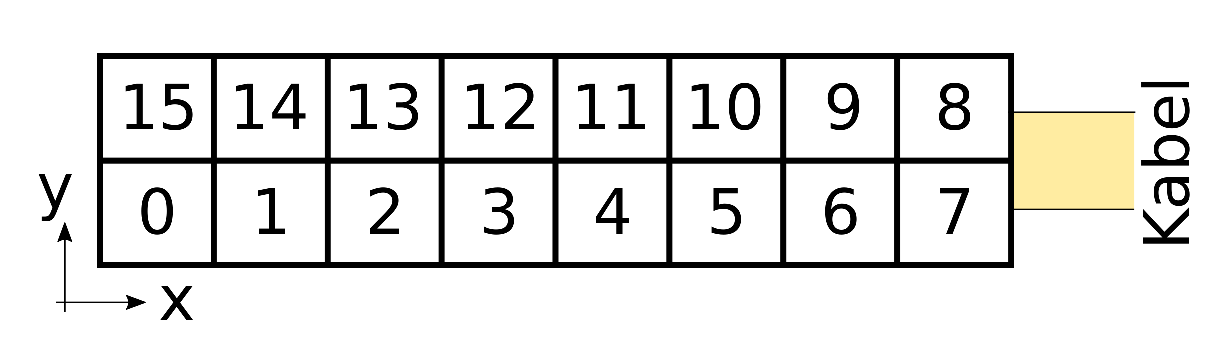
\includegraphics[width=0.7\textwidth]{fig/board.eps}
		\caption{Aufbau eines Boards mit 16 Pixel Chips. Jeder Pixel Chip besteht aus 52 x 80 einzelnen Pixeln und hat eine Größe von \SI{8100}{\micro\meter} x \SI{8100}{\micro\meter}}
		\label{fig:board}
	\end{figure}
	
	\begin{figure}
		\centering
	\subfigure[Erste Position der Quelle]{
	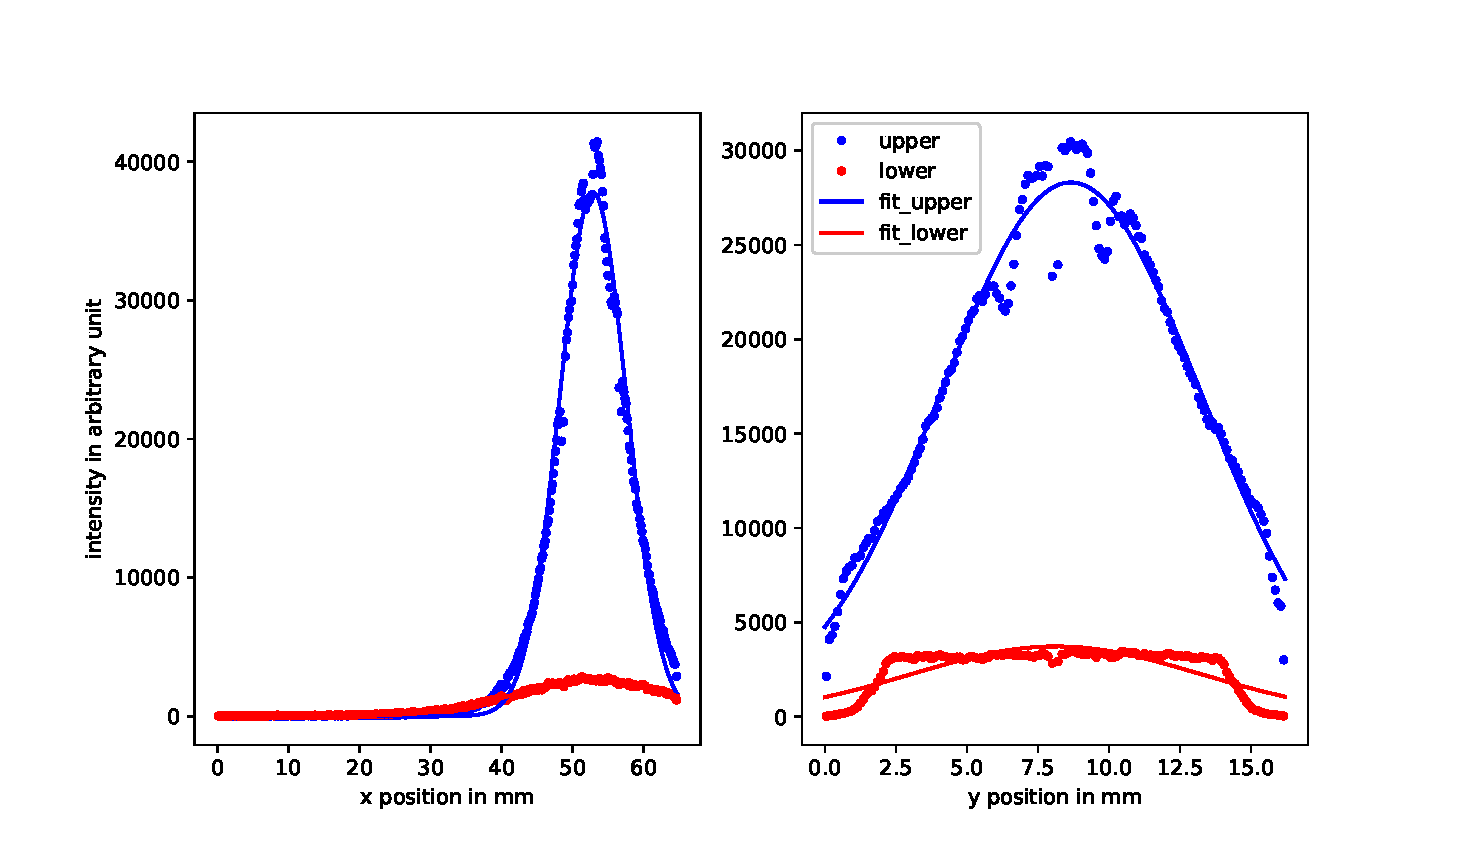
\includegraphics[width=\textwidth]{fig/alignment_1_fit.eps}}
	\label{fig:alignment_1}
	\subfigure[Zweite Position der Quelle]{
	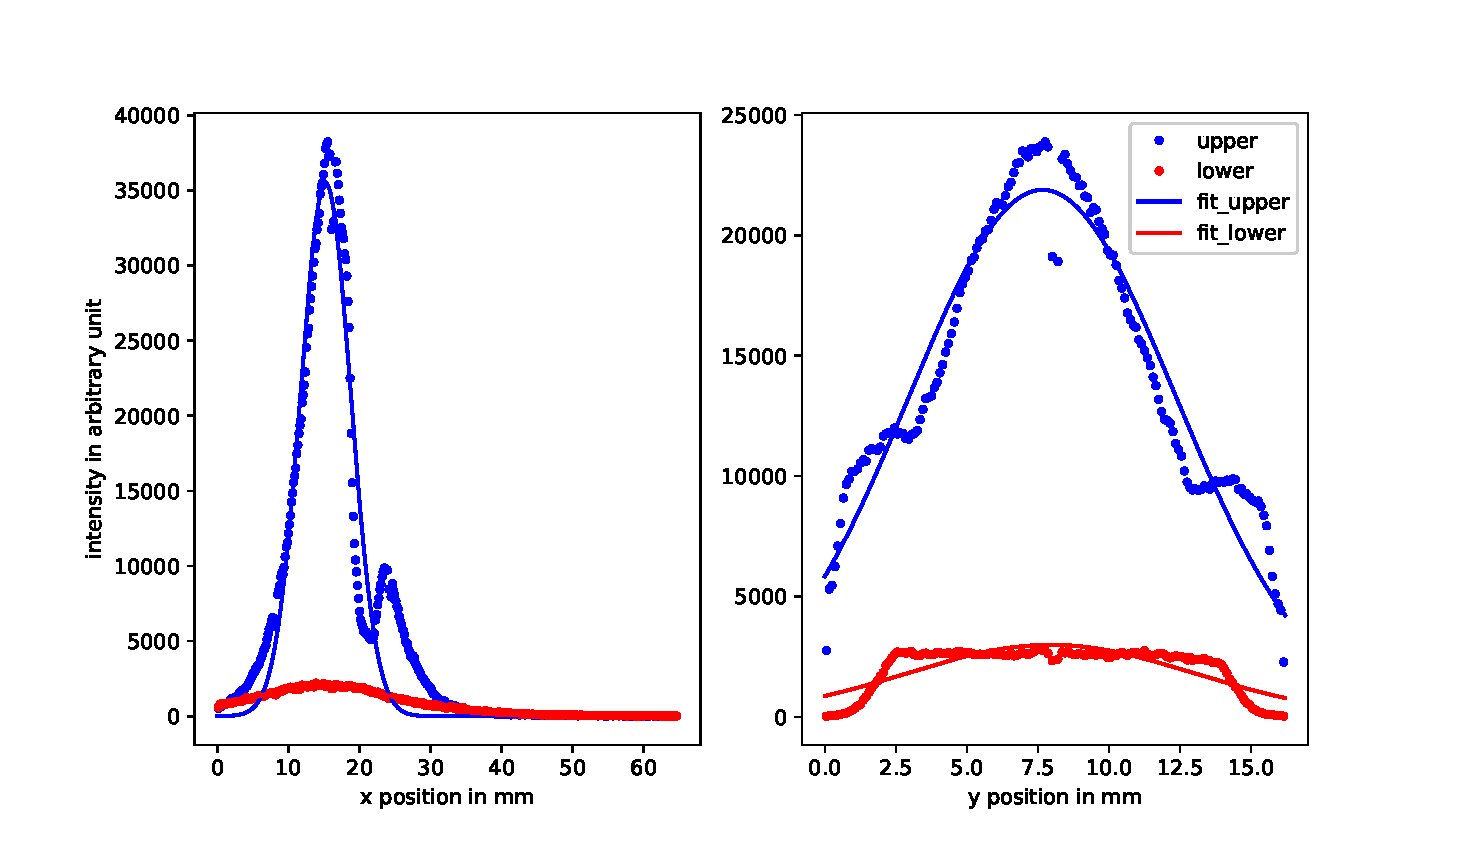
\includegraphics[width=\textwidth]{fig/alignment_2_fit.eps}}
	\label{fig:alignment_2}	
	\caption{Zur Bestimmung der Ausrichtung der beiden Boards zueinander wurde eine aktive Quelle an zwei unterschiedlichen Stellen auf dem Szintillator-Zähler positioniert.}
	\label{fig:alignment}
	\end{figure}

	Zur Bestimmung der Position der Quelle auf den Boards, wurden die Messwerte durch einen Gauss-Fit (Gl. \ref{eq:gauss}) approximiert - in Abbildung \ref{fig:alignment} als durchgezogene Linie dargestellt.
	
\begin{equation}
 	A\cdot e^{-\frac{(x-\mu)^{2}}{2\cdot \sigma^{2}}}
 	\label{eq:gauss}
\end{equation}
	
	Die Parameter für den besten Fit sind in Tabelle \ref{tab:alignment} aufgeführt.
	
	\xtable{htb}{alignment}{Fit Parameter für die Position der radioaktiven Quelle auf den Boards.}{} 
	
	
    %\chapter{Versuchsvorbereitung} 
    
    %\input{./chap/aufbau.tex}
   
    % appendix for more or less interesting calculations
    %\Appendix
    %\chapter*{\appendixname} \addcontentsline{toc}{chapter}{\appendixname}
    % to make the appendix appear in ToC without number. \appendixname = 
    % Appendix or Anhang (depending on chosen language)
    %\section{Messwerte}


\xtable{htb}{alignment}{Caption der Vorlage}{(Aufg. x.x)} 
 %\cleardoublepage

	\begingroup
	\let\clearpage\relax

    % Bibliography
    %\TheBibliography

    % BIBTEX
    % use if you want citations to appear even if they are not referenced to: 
    % \nocite{*} or maybe \nocite{Kon64,And59} for specific entries
    %\nocite{*}
    %\bibliographystyle{plain}
    %\bibliography{lit.bib}

    % THEBIBLIOGRAPHY
    %\begin{thebibliography}{000}
    %    \bibitem{ident}Entry into Bibliography.
    %\end{thebibliography}
    \endgroup
\end{document}
